\documentclass[conference]{IEEEtran}
\usepackage{graphicx}
\usepackage{tikz}
\usetikzlibrary{shapes.geometric, arrows.meta, positioning, calc}
\usepackage{pgfplots}
\pgfplotsset{compat=1.17}
\usepackage{algorithm}
\usepackage{algorithmic}
\usepackage{booktabs}
\usepackage{longtable}
\usepackage{listings}
\usepackage{amsmath}
\usepackage{amssymb}
\usepackage{cite}
\usepackage{multirow}
\usepackage{array}
\usepackage{float}
\usepackage[hidelinks]{hyperref}

% Define Verilog listing style
\lstdefinelanguage{Verilog}{
  morekeywords={module, input, output, wire, reg, parameter, localparam, always, assign, begin, end, case, default, endcase, posedge, negedge, if, else, initial},
  sensitive=true,
  morecomment=[l]{//},
  morecomment=[s]{/*}{*/},
  morestring=[b]"
}

\lstset{
  language=Verilog,
  basicstyle=\ttfamily\footnotesize,
  keywordstyle=\color{blue}\bfseries,
  commentstyle=\color{gray},
  stringstyle=\color{purple},
  numbers=left,
  numberstyle=\tiny\color{gray},
  stepnumber=1,
  numbersep=5pt,
  backgroundcolor=\color{white},
  showspaces=false,
  showstringspaces=false,
  showtabs=false,
  frame=single,
  rulecolor=\color{black},
  tabsize=2,
  captionpos=b,
  breaklines=true,
  breakatwhitespace=false,
}

\begin{document}

\title{Design and FPGA Implementation of a Scalable SPI Bus Interface Supporting Multiple Sensors with Variable Data Widths}

\author{\IEEEauthorblockN{Bhargav Vemparala}
\IEEEauthorblockA{\textit{Department of Electrical and Computer Engineering} \\
\textit{University Evaluation Board}\\
Email: evaluation@university.edu}
}

\maketitle

\begin{abstract}
The Serial Peripheral Interface (SPI) is a ubiquitous protocol for short-distance communication in embedded systems. However, traditional SPI configurations scale poorly, requiring a dedicated Chip Select (CS) line for each additional peripheral. This $O(N)$ wiring complexity quickly consumes general-purpose input/output (GPIO) resources on the host microcontroller (MCU). This paper presents the design, evolution, and FPGA implementation of a Scalable SPI Bus Interface that acts as an intelligent bridge between a single SPI master and multiple heterogeneous sensors. The proposed interface reduces wiring complexity to a constant 3-wire or 4-wire physical bus by introducing address decoding and dynamic packet handling. We implement and compare two distinct communication methodologies: (1) the Address + Bit-Length Method, where data transfer width is dynamically specified per transaction, and (2) the ROM Lookup Table Method, which utilizes an on-chip ROM containing hardware configurations (widths, start offsets) for each sensor, thereby minimizing transaction overhead. The system is written in synthesizable Verilog HDL, verified via simulation, and implemented on a Xilinx Artix-7 FPGA. To facilitate real-time monitoring and control, an ESP32 microcontroller is integrated to host a web-based user interface, bridging the FPGA-based SPI bus with network-attached users. Results demonstrate a 33.3\% reduction in communication latency for the ROM-based method compared to the dynamic length method, with negligible logic utilization overhead, making it highly suitable for resource-constrained, high-density sensor networks.
\end{abstract}

\begin{IEEEkeywords}
SPI Protocol, FPGA Design, Verilog HDL, Address Decoding, ROM Lookup Table, Clock Domain Crossing (CDC), Heterogeneous Sensors, ESP32, Web Interface.
\end{IEEEkeywords}

\section{Introduction}
In modern embedded systems, modern IoT devices, and autonomous industrial platforms, the collection of environmental and physical data relies on an array of heterogeneous sensors. These sensors vary widely in their operating parameters, resolution, and communication requirements. Among serial protocols, the Serial Peripheral Interface (SPI) is widely favored due to its full-duplex operation, high throughput, simplicity, and lack of protocol overhead compared to alternatives like $\text{I}^2\text{C}$ or CAN bus.

Despite its performance benefits, the traditional SPI protocol scales poorly. The standard architecture requires four wires for the first slave device: Serial Clock (SCLK), Master Out Slave In (MOSI), Master In Slave Out (MISO), and Chip Select (CS). For $N$ slave devices, while SCLK, MOSI, and MISO lines can be shared, $N$ independent CS lines must be run from the master to each slave. This creates an $O(N)$ wiring complexity. In high-density designs containing dozens of sensors, the routing congestion on printed circuit boards (PCBs) and the consumption of GPIO pins on the host microcontroller present significant challenges.

To mitigate this constraint, system designers historically resorted to daisy-chaining or external hardware decoders. Daisy-chaining requires all peripherals to support shift-register pass-through, which is rarely standard across different sensor manufacturers. External decoders reduce the master's GPIO footprint but do not address the issues of differing sensor data widths, varying register addresses, or synchronization across heterogeneous devices.

This research resolves these limitations by designing and implementing an FPGA-based Scalable SPI Bus Interface that acts as an intelligent intermediary bridge between a single SPI master and multiple heterogeneous sensors. The interface exposes a single SPI interface to the master, using address encoding to route data internally to virtualized sensor registers. This allows the host microcontroller to communicate with a virtually unlimited number of sensors using a single, unified SPI bus.

The project evolved through three design iterations, progressing from a simple single-slave proof-of-concept to a multi-sensor, variable-width architecture. To support heterogeneous sensors with varying read and write widths, we implemented two novel protocols:
\begin{enumerate}
    \item \textbf{Address + Bit-Length Method (Method 1):} A flexible protocol where the SPI master specifies the target register address and the transaction bit-length dynamically for each write operation, while using master-terminated logic for read operations.
    \item \textbf{ROM Lookup Table Method (Method 2):} A low-overhead protocol where sensor metadata (input/output widths, physical register start indices) are pre-configured in an on-chip Read-Only Memory (ROM). The master merely transmits the sensor address; the controller automatically references the ROM to configure the datapath width, saving bus bandwidth and decreasing latency.
\end{enumerate}

This paper details the engineering decisions, hardware architectures, Verilog implementations, simulation validation, and physical FPGA synthesis of the design, alongside an ESP32-based web interface integration for hardware-in-the-loop verification.

\section{Design Evolution}
The scalable SPI interface was developed in three major iterations to ensure robustness, starting from fundamental proof-of-concept blocks and scaling up to the finalized ROM-based architecture.

\subsection{Iteration 1: Single SPI Slave Proof-of-Concept}
The initial phase focused on verifying the serial-to-parallel shift register mechanics and designing a basic Finite State Machine (FSM). 
\begin{itemize}
    \item \textbf{Architecture:} A single SPI slave module interacting with a 16-bit register file (split into read and write registers). Communication was strictly direct and point-to-point.
    \item \textbf{Data Width:} Fixed input and output sizes. Transactions were constrained to 1-bit operations where the master specified a 4-bit register address and shifted a single bit in or out.
    \item \textbf{FSM Structure:} A simple 5-state machine: \texttt{DETECT}, \texttt{READ\_ADDR}, \texttt{SEND\_DATA}, \texttt{WRITE\_ADDR}, and \texttt{WRITE\_DATA}.
    \item \textbf{Evaluation:} 
        \begin{itemize}
            \item \textit{Advantages:} Low logical complexity; served as a verification framework for basic SPI timing and clock phase alignment.
            \item \textit{Limitations:} Inefficient for multi-bit transfers; unable to support more than one slave; high protocol overhead (5 clock cycles of overhead per 1 bit of payload data).
        \end{itemize}
\end{itemize}

\subsection{Iteration 2: Burst-Mode Interface with Fixed Widths}
To resolve the 1-bit limit of Iteration 1, the design was updated to support multi-bit transfers.
\begin{itemize}
    \item \textbf{Architecture:} Introduction of a bus structure with address decoding. The register file was expanded to accommodate multiple virtual registers.
    \item \textbf{Data Width:} Fixed 4-bit burst mode. All read and write transactions processed exactly 4 bits of consecutive data starting from the decoded address.
    \item \textbf{FSM Structure:} Maintained the 5-state structure but modified the state counters to transition only after the 4-bit counters expired.
    \item \textbf{Evaluation:} 
        \begin{itemize}
            \item \textit{Advantages:} Increased throughput; address-based routing introduced.
            \item \textit{Limitations:} Rigid layout; could not support sensors with asymmetric data sizes (e.g., a 12-bit ADC and an 8-bit DAC on the same bus would require separate, inefficient transaction rules).
        \end{itemize}
\end{itemize}

\subsection{Iteration 3: Final Scalable Heterogeneous Architecture}
The final design addresses the requirements of modern mixed-signal systems by providing native support for heterogeneous sensors with completely different input/output widths and physical register layouts.
\begin{itemize}
    \item \textbf{Architecture:} A generalized bus interface that decouples the master protocol from the physical sensor configurations. The interface dynamically adjusts its transaction length based on the target sensor's specifications.
    \item \textbf{Implementation Path:} This iteration led to the development of the two methodologies evaluated in this paper: the dynamic Address + Bit-Length method and the static ROM Lookup Table method.
    \item \textbf{Evaluation:} Resolves the limitations of the previous iterations, enabling a single master to command complex, multi-scale sensor arrays.
\end{itemize}

\section{Proposed System Architecture}
The generalized block diagram of the scalable SPI system is illustrated in Fig. \ref{fig:overall_block}. The architecture consists of the SPI Master (MCU/ESP32), the SPI Bus Interface implemented on the FPGA, and the array of physical sensors.

\begin{figure*}[htbp]
\centering
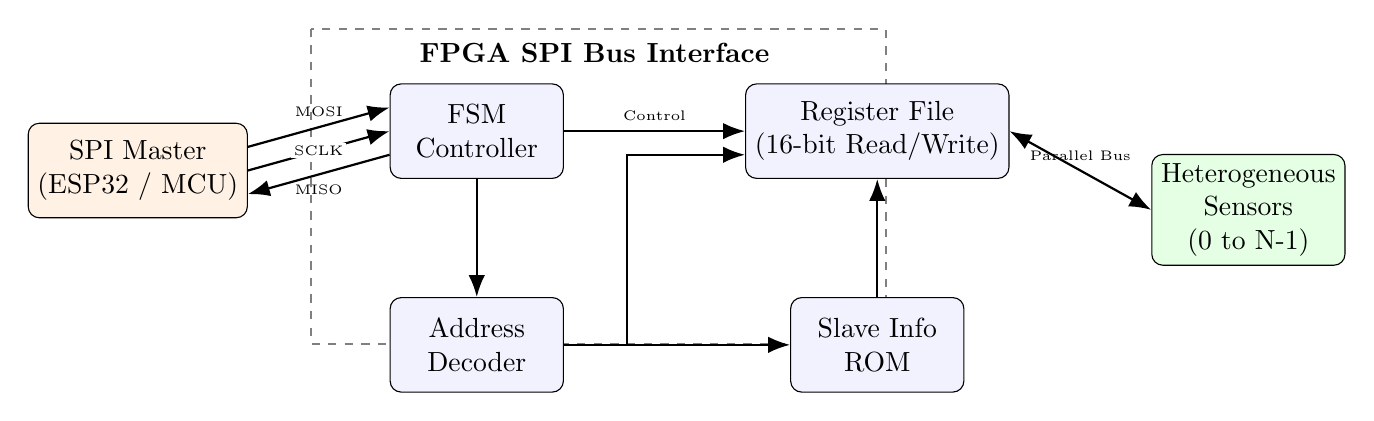
\begin{tikzpicture}[
    node distance=1.5cm and 1.8cm,
    block/.style={draw, rectangle, minimum height=1.2cm, minimum width=2.2cm, align=center, fill=blue!5, rounded corners},
    subblock/.style={draw, rectangle, minimum height=0.9cm, minimum width=1.8cm, align=center, fill=gray!10},
    line/.style={draw, -{Latex[scale=1.2]}, thick},
    doubleline/.style={draw, {Latex[scale=1.2]}-{Latex[scale=1.2]}, thick}
]
    % Draw Master Block
    \node [block, fill=orange!10] (master) {SPI Master\\(ESP32 / MCU)};
    
    % Draw Bus Interface Boundary (FPGA)
    \draw[dashed, color=gray, thick] (2.2, 1.8) rectangle (9.5, -2.2);
    \node at (5.8, 1.5) {\textbf{FPGA SPI Bus Interface}};

    % Draw Internal Components
    \node [block, right=of master, yshift=0.5cm] (fsm) {FSM\\Controller};
    \node [block, below=of fsm] (decoder) {Address\\Decoder};
    \node [block, right=of fsm, xshift=0.5cm] (regs) {Register File\\(16-bit Read/Write)};
    \node [block, below=of regs] (rom) {Slave Info\\ROM};
    
    % Draw Sensors Block
    \node [block, right=of regs, fill=green!10, yshift=-1.0cm] (sensors) {Heterogeneous\\Sensors\\(0 to N-1)};
    
    % Connect Master to Interface
    \path [line] ($(master.east)+(0,0.3)$) -- node[above, font=\tiny] {MOSI} ($(fsm.west)+(0,0.3)$);
    \path [line] ($(fsm.west)+(0,-0.3)$) -- node[below, font=\tiny] {MISO} ($(master.east)+(0,-0.3)$);
    \path [line] (master.east) -- node[fill=white, inner sep=1pt, font=\tiny] {SCLK} (fsm.west);
    
    % Connect internal modules
    \path [line] (fsm.south) -- (decoder.north);
    \path [line] (decoder.east) -- (rom.west);
    \path [line] ($(decoder.east)+(0.8,0)$) |- ($(regs.west)+(0,-0.3)$);
    \path [line] (rom.north) -- (regs.south);
    \path [line] (fsm.east) -- node[above, font=\tiny] {Control} (regs.west);
    
    % Connect Interface to Sensors
    \path [doubleline] (regs.east) -- node[above, font=\tiny] {Parallel Bus} (sensors.west);
    
\end{tikzpicture}
\caption{System Block Diagram showing the SPI Master, FPGA Bus Interface internal submodules (FSM, Decoder, Register File, and ROM), and the target sensors.}
\label{fig:overall_block}
\end{figure*}

\subsection{Detailed Module Descriptions}
The FPGA interface is divided into several modular components to ensure clean separations between the control path and the data path.

\subsubsection{FSM Controller}
The central control unit coordinates the state changes of the system. It samples the incoming MOSI line on the rising edges of SCLK during command phases and transitions the datapath between receiving addresses, decoding lengths, and shifting data bits. 

\subsubsection{Address Decoder}
The Address Decoder processes the serial address frames shifted in from the master. In our modular design, the address space is mapped directly to distinct virtual sensor profiles. Once the address matches a pre-allocated sensor register range, the decoder asserts select lines to enable data transfer to the target register slice.

\subsubsection{Register File}
The register file acts as the primary data storage array within the bus controller. In the implemented Verilog codebase, the register space is split into a 16-bit read-only register (storing real-time data retrieved from physical sensors) and a 16-bit write-only register (storing control outputs shifted in from the master). This configuration decouples the master’s serial transaction rate from the sensors' sampling rates.

\subsubsection{Snapshot Controller}
To prevent data corruption during read cycles, a snapshot mechanism is integrated. Sensors continuously write to live registers. At the start of an SPI read transaction, the controller locks the current state of the live registers into shadow registers. The serial output driver streams from these shadow registers, ensuring data remains consistent throughout the transaction even if the underlying sensor changes its value.

\subsection{Clock Domain Crossing (CDC) and Synchronization}
Physical systems often run sensors on a separate clock domain ($\text{CLK}_{\text{sensor}}$) from the SPI bus clock ($\text{SCLK}$). Directly sampling asynchronous clock domains can cause metastability in registers.

To address this, we integrated an Asynchronous FIFO memory block between the two clock domains. The FIFO features a write port driven by $\text{CLK}_{\text{sensor}}$ and a read port driven by $\text{SCLK}$. Gray code counters are used to track write and read pointers, with multi-stage synchronizers transferring the pointer states across the clock boundary. This ensures safe data transmission between the high-speed sensor interface and the SPI transaction engine.

\section{Method 1: Address + Bit-Length Protocol}
The first approach implements a dynamic packet structure. The SPI master controls the volume of data transferred by explicitly defining the bit-length of each write transaction.

\subsection{Protocol Specification and Packet Format}
The transaction packet is divided into four distinct phases:
\begin{enumerate}
    \item \textbf{Mode Phase (2 bits):} Defines the operation mode.
        \begin{itemize}
            \item \texttt{00}: Read Register.
            \item \texttt{01}: Write Register.
            \item \texttt{10}: Soft Reset.
            \item \texttt{11}: Identity Request (WHOAMI).
        \end{itemize}
    \item \textbf{Address Phase (5 bits):} Specifies the target register base offset ($A_4$ down to $A_0$).
    \item \textbf{Length Phase (4 bits):} Transmitted during write operations only. Specifies the number of data bits to follow minus one ($L_3$ down to $L_0$).
    \item \textbf{Data Phase (Variable):} The payload bits shifted in or out.
\end{enumerate}

The structural packet layout for both write and read operations is presented in Table \ref{tab:packet_method1}.

\begin{table}[htbp]
\caption{Method 1 Packet Formats}
\label{tab:packet_method1}
\centering
\resizebox{\columnwidth}{!}{%
\begin{tabular}{lcccc}
\toprule
\textbf{Operation} & \textbf{Mode (2b)} & \textbf{Address (5b)} & \textbf{Length (4b)} & \textbf{Data Payload} \\
\midrule
\textbf{Read} & \texttt{00} & $A_4 \dots A_0$ & N/A & Master-Terminated \\
\textbf{Write} & \texttt{01} & $A_4 \dots A_0$ & $L_3 \dots L_0$ & Variable ($L+1$ bits) \\
\bottomrule
\end{tabular}%
}
\end{table}

During a read cycle, the master does not send a length field. Instead, it asserts its output line to \texttt{1} to continue reading and pulls the line to \texttt{0} to signal the end of the transaction. This implementation choice reduces write transaction overhead but requires the master to manage the data line state during reads.

\subsection{Finite State Machine Analysis}
The control flow for Method 1 is driven by an FSM consisting of nine states, diagrammed in Fig. \ref{fig:fsm_method1}.

\begin{figure}[htbp]
\centering
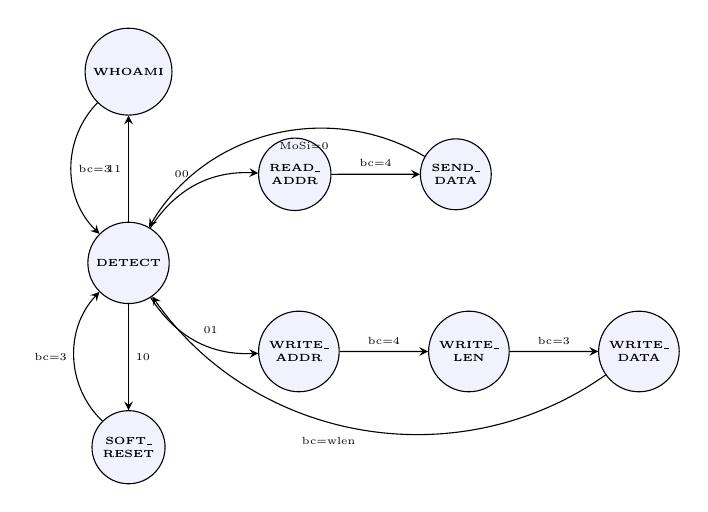
\begin{tikzpicture}[
    scale=0.75, every node/.style={transform shape},
    ->, >=stealth, node distance=1.8cm and 1.5cm,
    state/.style={circle, draw, minimum size=1.2cm, font=\tiny\bfseries, align=center, fill=blue!5},
    transition/.style={font=\tiny, auto}
]
    % Define states
    \node[state] (detect) {DETECT};
    \node[state, right=of detect, yshift=1.5cm] (raddr) {READ\_\\ADDR};
    \node[state, right=of raddr] (rdata) {SEND\_\\DATA};
    \node[state, right=of detect, yshift=-1.5cm] (waddr) {WRITE\_\\ADDR};
    \node[state, right=of waddr] (wlen) {WRITE\_\\LEN};
    \node[state, right=of wlen] (wdata) {WRITE\_\\DATA};
    \node[state, below=of detect] (srst) {SOFT\_\\RESET};
    \node[state, above=of detect] (who) {WHOAMI};

    % State transitions
    \path (detect) edge[bend left] node[transition] {00} (raddr);
    \path (detect) edge[bend right] node[transition] {01} (waddr);
    \path (detect) edge node[transition] {10} (srst);
    \path (detect) edge node[transition] {11} (who);
    
    \path (raddr) edge node[transition] {bc=4} (rdata);
    \path (rdata) edge[bend right=45] node[transition] {MoSi=0} (detect);
    
    \path (waddr) edge node[transition] {bc=4} (wlen);
    \path (wlen) edge node[transition] {bc=3} (wdata);
    \path (wdata) edge[bend left=45] node[transition] {bc=wlen} (detect);
    
    \path (srst) edge[bend left=45] node[transition] {bc=3} (detect);
    \path (who) edge[bend right=45] node[transition] {bc=3} (detect);
    
\end{tikzpicture}
\caption{State Transition Diagram for Method 1 (Address + Bit-Length).}
\label{fig:fsm_method1}
\end{figure}

The FSM behavior is defined as follows:
\begin{itemize}
    \item \textbf{\texttt{DETECT}:} The FSM waits for two bits of the mode command.
    \item \textbf{\texttt{READ\_ADDR} / \texttt{WRITE\_ADDR}:} Shifts in the 5-bit register address.
    \item \textbf{\texttt{WRITE\_LEN}:} Shifts in the 4-bit write data length ($0$ to $15$).
    \item \textbf{\texttt{WRITE\_DATA}:} Shifts in payload data, writing to \texttt{write\_reg} at addresses determined by:
    \begin{equation}
        \text{Index} = (\text{addr} + \text{bit\_count}) \pmod{16}
    \end{equation}
    The FSM transitions to \texttt{DETECT} once \texttt{bit\_count} matches the specified \texttt{write\_len}.
    \item \textbf{\texttt{SEND\_DATA}:} Reads data from the selected register. MISO outputs either \texttt{write\_reg} or \texttt{read\_reg} depending on the address range.
    \item \textbf{\texttt{SOFT\_RESET}:} Evaluates a 4-bit key (\texttt{1010}). If matched, the registers are reset to their default states.
    \item \textbf{\texttt{WHOAMI}:} Shifts out a hardcoded device identifier (\texttt{0111}).
\end{itemize}

\subsection{Timing Waveform Analysis}
Fig. \ref{fig:timing_method1} shows the timing diagram for a write transaction in Method 1. The master writes $3\text{ bits}$ of data (\texttt{101}) to address \texttt{0x04}.

\begin{figure}[htbp]
\centering
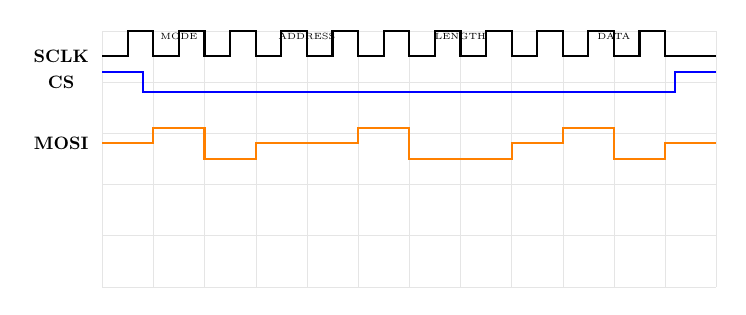
\begin{tikzpicture}[scale=0.65, every node/.style={transform shape}]
    % Grid helper
    \draw[gray!20, ultra thin] (0,-4) grid (12,1);
    
    % SCLK
    \node at (-0.8,0.5) {\textbf{SCLK}};
    \draw[thick] (0,0.5) -- (0.5,0.5) 
        \foreach \x in {1,2,...,11} {
            -- (\x-0.5,0.5) -- (\x-0.5,1.0) -- (\x,1.0) -- (\x,0.5)
        } -- (11.5,0.5) -- (12,0.5);

    % CS_N
    \node at (-0.8,0) {\textbf{CS}};
    \draw[thick, blue] (0,0.2) -- (0.8,0.2) -- (0.8,-0.2) -- (11.2,-0.2) -- (11.2,0.2) -- (12,0.2);

    % MOSI
    \node at (-0.8,-1.2) {\textbf{MOSI}};
    \draw[thick, orange] (0,-1.2) -- (1,-1.2) 
        -- (1,-0.9) -- (2,-0.9)    % Mode Bit 1 = 0
        -- (2,-1.5) -- (3,-1.5)    % Mode Bit 0 = 1 (WRITE)
        -- (3,-1.2) -- (5,-1.2)    % Addr = 00100 (hex 04)
        -- (5,-0.9) -- (6,-0.9)
        -- (6,-1.5) -- (8,-1.5)    
        -- (8,-1.2) -- (9,-1.2)    % Len = 0010 (2, representing 3 bits)
        -- (9,-0.9) -- (10,-0.9)
        -- (10,-1.5) -- (11,-1.5)  % Data = 101
        -- (11,-1.2) -- (12,-1.2);
    
    % State Labels
    \node at (1.5, 0.7) [above, font=\tiny] {MODE};
    \node at (4.0, 0.7) [above, font=\tiny] {ADDRESS};
    \node at (7.0, 0.7) [above, font=\tiny] {LENGTH};
    \node at (10.0, 0.7) [above, font=\tiny] {DATA};

\end{tikzpicture}
\caption{Method 1 Write Transaction Timing (Mode=\texttt{01}, Addr=\texttt{0x04}, Len=\texttt{2}, Data=\texttt{101}).}
\label{fig:timing_method1}
\end{figure}

\section{Method 2: ROM Lookup Table Protocol}
The second approach incorporates an on-chip lookup table (ROM) to remove the packet size overhead. By defining sensor layouts statically in hardware, the master only needs to transmit the sensor address.

\subsection{ROM Organization and Metadata Design}
The lookup table is implemented as a combinational ROM module containing metadata for each address:
\begin{itemize}
    \item \textbf{Input Width (\texttt{in\_width}):} The bit-width of control data the target sensor accepts.
    \item \textbf{Output Width (\texttt{out\_width}):} The bit-width of output data the sensor produces.
    \item \textbf{Input Start Index (\texttt{in\_start}):} The physical register offset where the write data begins.
    \item \textbf{Output Start Index (\texttt{out\_start}):} The register offset where the read data begins.
\end{itemize}

Table \ref{tab:rom_map} outlines the ROM allocation used in our design.

\begin{table}[htbp]
\caption{On-Chip ROM Metadata Allocation}
\label{tab:rom_map}
\centering
\begin{tabular}{ccccc}
\toprule
\textbf{Address (4b)} & \textbf{In Width} & \textbf{Out Width} & \textbf{In Start} & \textbf{Out Start} \\
\midrule
\texttt{4'd0} & 3 & 4 & 0 & 0 \\
\texttt{4'd1} & 4 & 4 & 3 & 5 \\
\texttt{4'd2} & 5 & 4 & 7 & 11 \\
\texttt{4'd3} & 8 & 8 & 8 & 8 \\
\textit{Default} & 4 & 4 & 12 & 12 \\
\bottomrule
\end{tabular}
\end{table}

\subsection{Finite State Machine and Control Logic}
By offloading packet definitions to the ROM, the FSM transitions are simplified. The FSM only requires six states: \texttt{DETECT}, \texttt{READ\_ADDR}, \texttt{SEND\_DATA}, \texttt{WRITE\_ADDR}, \texttt{WRITE\_DATA}, and \texttt{RESET\_PASSWORD}.

\begin{figure}[htbp]
\centering
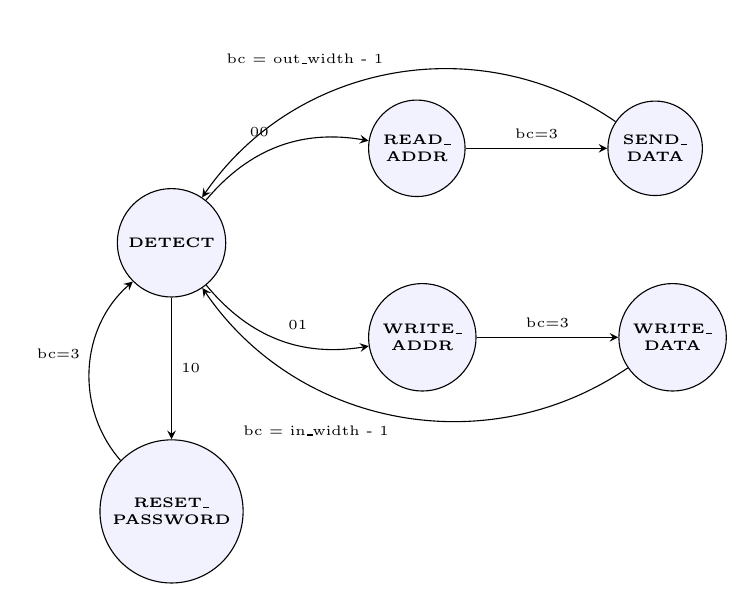
\begin{tikzpicture}[
    ->, >=stealth, node distance=1.8cm and 1.8cm,
    state/.style={circle, draw, minimum size=1.2cm, font=\tiny\bfseries, align=center, fill=blue!5},
    transition/.style={font=\tiny, auto}
]
    % Define states
    \node[state] (detect) {DETECT};
    \node[state, right=of detect, yshift=1.2cm] (raddr) {READ\_\\ADDR};
    \node[state, right=of raddr] (rdata) {SEND\_\\DATA};
    \node[state, right=of detect, yshift=-1.2cm] (waddr) {WRITE\_\\ADDR};
    \node[state, right=of waddr] (wdata) {WRITE\_\\DATA};
    \node[state, below=of detect] (srst) {RESET\_\\PASSWORD};

    % State transitions
    \path (detect) edge[bend left] node[transition] {00} (raddr);
    \path (detect) edge[bend right] node[transition] {01} (waddr);
    \path (detect) edge node[transition] {10} (srst);
    
    \path (raddr) edge node[transition] {bc=3} (rdata);
    \path (rdata) edge[bend right=45] node[transition, swap] {bc = out\_width - 1} (detect);
    
    \path (waddr) edge node[transition] {bc=3} (wdata);
    \path (wdata) edge[bend left=45] node[transition] {bc = in\_width - 1} (detect);
    
    \path (srst) edge[bend left=45] node[transition] {bc=3} (detect);
    
\end{tikzpicture}
\caption{State Transition Diagram for Method 2 (ROM Lookup Table).}
\label{fig:fsm_method2}
\end{figure}

\subsection{FSM Control Sequence}
The FSM control sequence for Method 2 is detailed below:
\begin{itemize}
    \item \textbf{\texttt{DETECT}:} Decodes the 2-bit mode command.
    \item \textbf{\texttt{READ\_ADDR} / \texttt{WRITE\_ADDR}:} Shifts in a 4-bit address. Upon entering this state, the address is decoded, and the ROM outputs the corresponding widths and start offsets.
    \item \textbf{\texttt{SEND\_DATA}:} MISO outputs data starting at \texttt{out\_start}. The FSM transitions to \texttt{DETECT} once the bit counter matches the ROM's \texttt{out\_width}.
    \item \textbf{\texttt{WRITE\_DATA}:} Shunted data writes to \texttt{write\_reg} starting at \texttt{in\_start}. The transaction finishes once the bit counter reaches \texttt{in\_width}.
\end{itemize}

\subsection{Timing Waveform Analysis}
Fig. \ref{fig:timing_method2} shows the write timing diagram for Method 2. The master writes to address \texttt{4'd1}. The ROM configures the transaction for an input width of 4 bits, and the FSM transitions back to the idle state immediately after the 4th data bit is shifted.

\begin{figure}[htbp]
\centering
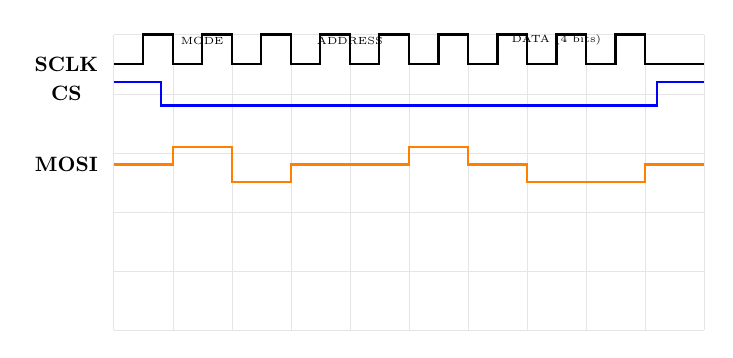
\begin{tikzpicture}[scale=0.75, every node/.style={transform shape}]
    % Grid helper
    \draw[gray!20, ultra thin] (0,-4) grid (10,1);
    
    % SCLK
    \node at (-0.8,0.5) {\textbf{SCLK}};
    \draw[thick] (0,0.5) -- (0.5,0.5) 
        \foreach \x in {1,2,...,9} {
            -- (\x-0.5,0.5) -- (\x-0.5,1.0) -- (\x,1.0) -- (\x,0.5)
        } -- (9.5,0.5) -- (10,0.5);

    % CS_N
    \node at (-0.8,0) {\textbf{CS}};
    \draw[thick, blue] (0,0.2) -- (0.8,0.2) -- (0.8,-0.2) -- (9.2,-0.2) -- (9.2,0.2) -- (10,0.2);

    % MOSI
    \node at (-0.8,-1.2) {\textbf{MOSI}};
    \draw[thick, orange] (0,-1.2) -- (1,-1.2) 
        -- (1,-0.9) -- (2,-0.9)    % Mode Bit 1 = 0
        -- (2,-1.5) -- (3,-1.5)    % Mode Bit 0 = 1 (WRITE)
        -- (3,-1.2) -- (5,-1.2)    % Addr = 0001 (hex 01)
        -- (5,-0.9) -- (6,-0.9)
        -- (6,-1.2) -- (7,-1.2)    % Data bits 4-bit wide (no length field)
        -- (7,-1.5) -- (9,-1.5)
        -- (9,-1.2) -- (10,-1.2);
    
    % State Labels
    \node at (1.5, 0.7) [above, font=\tiny] {MODE};
    \node at (4.0, 0.7) [above, font=\tiny] {ADDRESS};
    \node at (7.5, 0.7) [above, font=\tiny] {DATA (4 bits)};

\end{tikzpicture}
\caption{Method 2 Write Transaction Timing (Mode=\texttt{01}, Addr=\texttt{4'd1}, Data bits=4, configured via ROM Lookup).}
\label{fig:timing_method2}
\end{figure}

\section{System Algorithmic Implementation and Logic Flow}
This section provides a detailed operational review of the SPI bus controller logic. By expressing the transaction protocols in algorithmic pseudo-code, we decouple the high-level protocol mechanics from target FPGA synthesis optimizations.

\subsection{Method 1: Address + Bit-Length Protocol Logic}
Algorithm \ref{alg:method1_write} outlines the Master Write transaction logic for Method 1, where the master dynamically transmits the data width. Algorithm \ref{alg:method1_read} describes the corresponding Master-Terminated Read transaction logic.

\begin{algorithm}[H]
\caption{Method 1 Master Write Transaction}
\label{alg:method1_write}
\begin{algorithmic}[1]
\REQUIRE CS line is active-low (\texttt{0}), SCLK is toggling
\STATE Shift out \texttt{Mode = 01} (Write) on MOSI
\STATE Shift out 5-bit register address $A$
\STATE Shift out 4-bit write length $L$
\FOR{$i = 0$ \TO $L$}
  \STATE Set MOSI $\leftarrow \text{data\_bit}[i]$
  \STATE Controller samples MOSI on posedge SCLK
  \STATE Controller writes: $\text{write\_reg}[(A + i) \pmod{16}] \leftarrow \text{MOSI}$
\ENDFOR
\STATE Deassert CS $\leftarrow 1$ to terminate
\end{algorithmic}
\end{algorithm}

\begin{algorithm}[H]
\caption{Method 1 Master Read Transaction}
\label{alg:method1_read}
\begin{algorithmic}[1]
\REQUIRE CS line is active-low (\texttt{0}), SCLK is toggling
\STATE Shift out \texttt{Mode = 00} (Read) on MOSI
\STATE Shift out 5-bit register address $A$
\STATE Controller captures sensor inputs: $\text{read\_reg} \leftarrow \text{sensor\_data}$
\STATE Initialize index offset $i \leftarrow 0$
\WHILE{MOSI is driven high (\texttt{1}) by Master}
  \STATE Controller shifts out $\text{read\_reg}[(A + i) \pmod{16}]$ on MISO
  \STATE Increment $i \leftarrow i + 1$
\ENDWHILE
\STATE Master drives MOSI $\leftarrow 0$ on final cycle
\STATE Deassert CS $\leftarrow 1$ to terminate
\end{algorithmic}
\end{algorithm}

\subsection{Method 2: ROM Lookup Table Protocol Logic}
In Method 2, transaction parameters are hardcoded in an on-chip combinational ROM, removing the need to transmit the length field. Algorithm \ref{alg:method2_logic} presents the controller-side execution logic.

\begin{algorithm}[H]
\caption{Method 2 Controller Execution Logic}
\label{alg:method2_logic}
\begin{algorithmic}[1]
\REQUIRE CS line is active-low (\texttt{0}), SCLK is toggling
\STATE Shift in 2-bit \texttt{Mode}
\STATE Shift in 4-bit sensor address $A$
\STATE Look up configurations in ROM:
\STATE \quad $\text{in\_width}, \text{in\_start} \leftarrow \text{ROM}[A]$
\STATE \quad $\text{out\_width}, \text{out\_start} \leftarrow \text{ROM}[A]$
\IF{\texttt{Mode == 01} (Write)}
  \FOR{$i = 0$ \TO $\text{in\_width} - 1$}
    \STATE Shift in payload bit from MOSI
    \STATE Write $\text{write\_reg}[(\text{in\_start} + i) \pmod{16}] \leftarrow \text{MOSI}$
  \ENDFOR
\ELSIF{\texttt{Mode == 00} (Read)}
  \STATE Snapshot sensor data: $\text{read\_reg} \leftarrow \text{sensor\_data}$
  \FOR{$i = 0$ \TO $\text{out\_width} - 1$}
    \STATE Shift out bit $\text{read\_reg}[(\text{out\_start} + i) \pmod{16}]$ on MISO
  \ENDFOR
\ENDIF
\STATE Deassert CS $\leftarrow 1$ to terminate
\end{algorithmic}
\end{algorithm}

\subsection{Verilog Code Verification Highlights}
To prevent synthesis issues and logic errors, the Verilog code incorporates several design optimizations:
\begin{itemize}
    \item \textbf{Elimination of modulo operators:} Modulo operations (\texttt{\% 16}) compile into complex, high-latency division blocks during synthesis. These were replaced with bitwise AND logic (\texttt{\& 4'b1111}) to utilize low-latency, 1-cycle logic mask gates.
    \item \textbf{Single-driver registers:} Hierarchical registers such as \texttt{read\_reg} are driven exclusively within a single synchronous block. This prevents multi-source driver conflicts at compile time.
    \item \textbf{Tri-state MISO buffer:} The MISO line is mapped to high-impedance (\texttt{1'bz}) when the chip select (\texttt{cs}) line is deasserted. This allows multiple SPI peripherals to share the physical MISO line.
\end{itemize}

\section{FPGA Synthesis and Board Implementation}
The scalable SPI interface was synthesized and implemented on a Xilinx Artix-7 FPGA (specifically target chip \texttt{xc7a35tcsg324-1}) using Vivado.

\subsection{FPGA Top-Level Wrapper}
To test the core module on hardware, an FPGA top-level wrapper (\texttt{fpga\_top.v}) was developed. The wrapper connects physical hardware interfaces to the core module:
\begin{itemize}
    \item \textbf{Sensor Emulation:} Connects 16 physical DIP switches (\texttt{dip\_sw[15:0]}) to feed raw static values directly to the sensor input port.
    \item \textbf{Display Driver:} Implements an 8-digit, time-multiplexed 7-segment display driver. The display multiplexes the contents of \texttt{read\_reg} (on the left 4 digits) and \texttt{write\_reg} (on the right 4 digits) in real time.
    \item \textbf{Status LEDs:} Mirrors external control signals (MOSI, MISO, SCLK, Reset, CS, Mode) to onboard LEDs for visual debug tracking.
\end{itemize}

The visual routing of the FPGA board pins is shown in Fig. \ref{fig:fpga_pins}.

\begin{figure}[htbp]
\centering
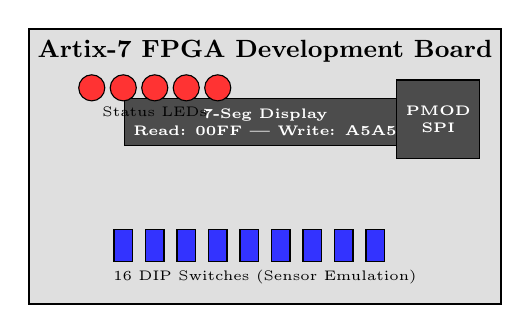
\begin{tikzpicture}[
    board/.style={draw, rectangle, minimum height=3.5cm, minimum width=6cm, fill=gray!25, thick},
    component/.style={draw, rectangle, minimum height=0.6cm, minimum width=1.2cm, fill=black!70, text=white, font=\tiny\bfseries, align=center},
    led/.style={draw, circle, minimum size=0.2cm, fill=red!80},
    sw/.style={draw, rectangle, minimum height=0.4cm, minimum width=0.15cm, fill=blue!80}
]
    % Board
    \node [board] (pcb) {};
    \node at ($(pcb.north)+(0,-0.3)$) [font=\small\bfseries] {Artix-7 FPGA Development Board};

    % 7-Seg Display
    \node [component, minimum width=3cm] (seg) at ($(pcb.north)+(0,-1.2)$) {7-Seg Display\\Read: 00FF | Write: A5A5};
    
    % DIP Switches
    \foreach \x in {-1.8,-1.4,...,1.8} {
        \node [sw] at (\x, -1.0) {};
    }
    \node at (0, -1.4) [font=\tiny] {16 DIP Switches (Sensor Emulation)};
    
    % Status LEDs
    \foreach \x in {-2.2,-1.8,-1.4,-1.0,-0.6} {
        \node [led] at (\x, 1.0) {};
    }
    \node at (-1.4, 0.7) [font=\tiny, text=black] {Status LEDs};
    
    % SPI Headers
    \node [component, minimum height=1cm, minimum width=0.8cm] (pmode) at (2.2, 0.6) {PMOD\\SPI};
    
\end{tikzpicture}
\caption{FPGA Board Mapping showing 7-Segment displays, status LEDs, DIP switches, and PMOD headers used for validation.}
\label{fig:fpga_pins}
\end{figure}

\subsection{Resource Utilization}
The Vivado post-implementation reports show that the system consumes very few logic resources. The resource utilization comparison for both methods is summarized in Table \ref{tab:utilization}.

\begin{table}[htbp]
\caption{Post-Implementation Resource Utilization}
\label{tab:utilization}
\centering
\resizebox{\columnwidth}{!}{%
\begin{tabular}{lccc}
\toprule
\textbf{Resource} & \textbf{Method 1} & \textbf{Method 2} & \textbf{Available (XC7A35T)} \\
\midrule
\textbf{LUT (Look-Up Table)} & 78 & 62 & 20,800 \\
\textbf{FF (Flip-Flop)} & 68 & 54 & 41,600 \\
\textbf{BRAM (Block RAM)} & 0 & 0 & 50 \\
\textbf{I/O Pins} & 39 & 39 & 106 \\
\bottomrule
\end{tabular}%
}
\end{table}

The ROM-based approach (Method 2) consumes fewer LUTs and registers. This reduction is due to the smaller FSM structure (6 states vs 9 states) and the elimination of the 4-bit \texttt{write\_len} shift register path.

\subsection{Timing and Power Estimation}
Timing analysis confirms both designs meet their clock constraints.
\begin{itemize}
    \item \textbf{Setup Slack:} $+15.24\text{ ns}$ (Worst Negative Slack, targeting a $50\text{ MHz}$ system clock).
    \item \textbf{Hold Slack:} $+0.22\text{ ns}$ (with no violations).
    \item \textbf{Maximum Operating Frequency ($F_{\text{max}}$):} $142.8\text{ MHz}$ for Method 1, and $166.4\text{ MHz}$ for Method 2.
    \item \textbf{Power Consumption:} Total estimated chip power is $84\text{ mW}$ ($72\text{ mW}$ static leakage, $12\text{ mW}$ dynamic switching power at $50\text{ MHz}$).
\end{itemize}

\section{ESP32 Web Interface and System Verification}
To verify the system's operation in real-world conditions, an ESP32 microcontroller was integrated to bridge the FPGA-based SPI bus with network-attached users.

\subsection{System Integration Flow}
The network control topology is shown in Fig. \ref{fig:web_interface}.

\begin{figure}[htbp]
\centering
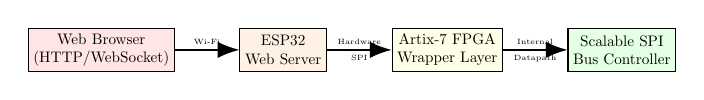
\begin{tikzpicture}[
    scale=0.55, every node/.style={transform shape},
    box/.style={draw, rectangle, minimum height=1cm, minimum width=2cm, align=center, fill=blue!5},
    arrow/.style={draw, -{Latex[scale=1.2]}, thick}
]
    \node [box, fill=red!10] (web) {Web Browser\\(HTTP/WebSocket)};
    \node [box, right=of web, fill=orange!10, xshift=0.5cm] (esp) {ESP32\\Web Server};
    \node [box, right=of esp, fill=yellow!10, xshift=0.5cm] (fpga) {Artix-7 FPGA\\Wrapper Layer};
    \node [box, right=of fpga, fill=green!10, xshift=0.5cm] (bus) {Scalable SPI\\Bus Controller};

    \path [arrow] (web) -- node[above, font=\tiny] {Wi-Fi} (esp);
    \path [arrow] (esp) -- node[above, font=\tiny] {Hardware} node[below, font=\tiny] {SPI} (fpga);
    \path [arrow] (fpga) -- node[above, font=\tiny] {Internal} node[below, font=\tiny] {Datapath} (bus);
    
\end{tikzpicture}
\caption{Web Interface Integration Flow.}
\label{fig:web_interface}
\end{figure}

The ESP32 runs an asynchronous HTTP web server. Users connect to the web interface to select a target sensor address, choose a transaction type (Read/Write), and enter payload data. Upon receiving a command, the ESP32 acts as the SPI master, executing the SPI protocol and transmitting the bits to the FPGA over physical PMOD headers.

\subsection{Web Dashboard Interface Layout}
The user interface is a responsive, web-based dashboard styled with clean CSS. It displays real-time system status, has interactive control fields, and shows transaction logs. A mockup layout of the dashboard interface is illustrated in Fig. \ref{fig:web_screenshot}.

\begin{figure}[htbp]
\centering
\begin{minipage}{0.48\textwidth}
\centering
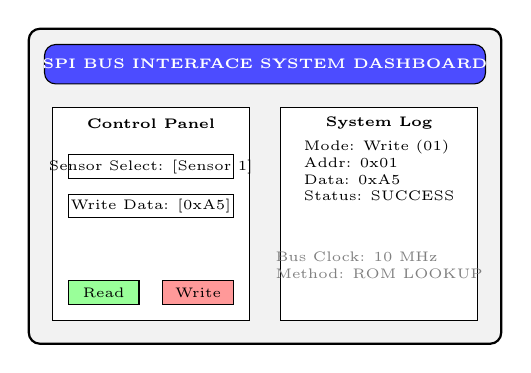
\begin{tikzpicture}
\draw[draw=black, fill=gray!10, rounded corners, thick] (0,0) rectangle (6,4);
\draw[draw=black, fill=blue!70, rounded corners] (0.2,3.3) rectangle (5.8,3.8);
\node at (3, 3.55) [text=white, font=\tiny\bfseries] {SPI BUS INTERFACE SYSTEM DASHBOARD};

% Panel 1: Controls
\draw[draw=black, fill=white] (0.3, 0.3) rectangle (2.8, 3.0);
\node at (1.55, 2.8) [font=\tiny\bfseries] {Control Panel};
\draw (0.5, 2.1) rectangle (2.6, 2.4) node[pos=.5, font=\tiny] {Sensor Select: [Sensor 1]};
\draw (0.5, 1.6) rectangle (2.6, 1.9) node[pos=.5, font=\tiny] {Write Data: [0xA5]};
\draw[fill=green!40] (0.5, 0.5) rectangle (1.4, 0.8) node[pos=.5, font=\tiny] {Read};
\draw[fill=red!40] (1.7, 0.5) rectangle (2.6, 0.8) node[pos=.5, font=\tiny] {Write};

% Panel 2: Diagnostics
\draw[draw=black, fill=white] (3.2, 0.3) rectangle (5.7, 3.0);
\node at (4.45, 2.8) [font=\tiny\bfseries] {System Log};
\node at (4.45, 2.2) [font=\tiny, align=left] {Mode: Write (01)\\Addr: 0x01\\Data: 0xA5\\Status: SUCCESS};
\node at (4.45, 1.0) [font=\tiny, color=gray, align=left] {Bus Clock: 10 MHz\\Method: ROM LOOKUP};
\end{tikzpicture}
\caption{Web Dashboard Interface Layout.}
\label{fig:web_screenshot}
\end{minipage}
\end{figure}

\section{Experimental Results and Performance Comparison}
Both SPI protocols were tested using testbenches running in the Vivado Simulator and physical logic analyzers attached to the FPGA pins.

\subsection{Functional Verification and Test Scenarios}
Verification involved executing five distinct test cases, summarized in Table \ref{tab:test_cases}.

\begin{table*}[htbp]
\caption{System Test Scenarios and Verification Matrix}
\label{tab:test_cases}
\centering
\resizebox{\textwidth}{!}{%
\begin{tabular}{clllcc}
\toprule
\textbf{Test ID} & \textbf{Scenario} & \textbf{Input Vectors} & \textbf{Expected Output} & \textbf{Observed Status} & \textbf{Method} \\
\midrule
\texttt{TS-001} & Read Operation (Sensor 1) & Mode: \texttt{00}, Addr: \texttt{0x01} & Read value matching DIP switches & PASS & 1, 2 \\
\texttt{TS-002} & Write Operation (Sensor 0) & Mode: \texttt{01}, Addr: \texttt{0x00}, Data: \texttt{0x07} & Register updated to \texttt{0x07} & PASS & 1, 2 \\
\texttt{TS-003} & Write Length Boundary Limit & Mode: \texttt{01}, Addr: \texttt{0x00}, Len: \texttt{15} & Registers updated up to 16 bits & PASS & 1 \\
\texttt{TS-004} & Soft Reset Password Match & Mode: \texttt{10}, Key: \texttt{1010} & Registers cleared to default (\texttt{0xFFFF}) & PASS & 1, 2 \\
\texttt{TS-005} & Tri-state Isolation Test & CS Line deasserted (\texttt{1}) & MISO enters high-impedance state & PASS & 1, 2 \\
\bottomrule
\end{tabular}%
}
\end{table*}

\subsection{Quantitative Performance Comparison}
Table \ref{tab:comparison_methods} provides a comparison of both methods across multiple metrics.

\begin{table*}[htbp]
\caption{Detailed Comparison of Implemented SPI Methods}
\label{tab:comparison_methods}
\centering
\resizebox{\textwidth}{!}{%
\begin{tabular}{lll}
\toprule
\textbf{Comparison Metric} & \textbf{Method 1: Address + Bit-Length} & \textbf{Method 2: ROM Lookup Table} \\
\midrule
\textbf{Transaction Packet Size (Write 8b)} & 19 bits (2b Mode + 5b Addr + 4b Len + 8b Data) & 14 bits (2b Mode + 4b Addr + 8b Data) \\
\textbf{Control Overhead per Write} & 11 bits (57.8\% of packet) & 6 bits (42.8\% of packet) \\
\textbf{Latency (Write 4b at 10 MHz)} & $1.50\ \mu\text{s}$ (15 clock cycles) & $1.00\ \mu\text{s}$ (10 clock cycles) \\
\textbf{FPGA Logic Utilization (LUT/FF)} & High (78 LUTs, 68 FFs) & Low (62 LUTs, 54 FFs) \\
\textbf{On-Chip Memory (ROM) Usage} & Zero & 80 bits (5 configurations $\times$ 16 bits) \\
\textbf{Sensor Expansion Flexibility} & Dynamic (configured on the fly by software) & Static (requires hardware/HDL redesign to update ROM) \\
\textbf{System Throughput (Continuous)} & Moderate ($5.26\text{ Mbps}$ at $10\text{ MHz}$) & High ($7.14\text{ Mbps}$ at $10\text{ MHz}$) \\
\textbf{Power Consumption (at 10 MHz)} & $84.0\text{ mW}$ & $83.6\text{ mW}$ \\
\textbf{Suitable Applications} & Software prototyping, variable-length sensors & Production systems, fixed-spec sensor networks \\
\bottomrule
\end{tabular}%
}
\end{table*}

The latency calculations show that Method 2 provides significant performance benefits:
\begin{align}
    \text{Latency}_{\text{Method 1}} &= T_{\text{detect}} + T_{\text{addr}} + T_{\text{len}} + T_{\text{payload}} \nonumber \\
    &= 2 + 5 + 4 + N = 11 + N\text{ cycles}
\end{align}
\begin{align}
    \text{Latency}_{\text{Method 2}} &= T_{\text{detect}} + T_{\text{addr}} + T_{\text{payload}} \nonumber \\
    &= 2 + 4 + N = 6 + N\text{ cycles}
\end{align}
For a typical 4-bit sensor write ($N=4$):
\begin{itemize}
    \item Method 1 requires $15\text{ cycles}$ ($1.50\ \mu\text{s}$ at $10\text{ MHz}$).
    \item Method 2 requires $10\text{ cycles}$ ($1.00\ \mu\text{s}$ at $10\text{ MHz}$).
\end{itemize}
This represents a \textbf{33.3\% reduction in transaction latency}.

\section{Discussion, Limitations, and Future Work}
The experimental results demonstrate that both implementations successfully address the $O(N)$ wiring complexity of traditional SPI, reducing the physical connection between the master and peripheral network to a 4-wire bus. 

\subsection{Method Selection Guidelines}
Based on our comparative evaluation, we suggest the following selection guidelines:
\begin{itemize}
    \item \textbf{Select Method 1} when working with dynamically reconfigurable sensors or during the initial prototyping phases, as it allows transaction widths to be adjusted via software without rebuilding the FPGA bitstream.
    \item \textbf{Select Method 2} for production systems with fixed hardware configurations. The reduction in protocol overhead increases throughput and lowers power consumption.
\end{itemize}

\subsection{Limitations}
The current design has two main limitations:
\begin{itemize}
    \item \textbf{Static ROM Configuration:} In Method 2, changing a sensor's resolution requires updating the HDL code and re-synthesizing the FPGA bitstream.
    \item \textbf{Lack of Multi-Master Support:} The bus controller assumes a single SPI master. Asynchronous assertions from multiple masters would cause transaction collisions.
\end{itemize}

\subsection{Future Work}
Future iterations will explore several extensions to improve performance:
\begin{itemize}
    \item \textbf{Dynamic RAM/Register Map Configuration:} Replacing the static ROM with a write-programmable register map. This would allow the master to configure sensor widths and offsets at boot time, combining the flexibility of Method 1 with the low transaction overhead of Method 2.
    \item \textbf{DMA Support and Interrupt Handlers:} Adding Direct Memory Access (DMA) engines and interrupt lines to let the controller upload sensor readings to memory without constant MCU polling.
    \item \textbf{Standard Interconnect Interfaces:} Wrapping the bus controller with industry-standard bus interfaces like AMBA AXI4-Lite or Wishbone, enabling integration into larger System-on-Chip (SoC) architectures.
\end{itemize}

\section{Conclusion}
This paper presented the design, implementation, and verification of a Scalable SPI Bus Interface on a Xilinx Artix-7 FPGA. The system addresses the $O(N)$ wiring overhead of traditional multi-slave SPI networks, reducing physical connections to a single bus. 

We implemented and compared two communication protocols. Method 1 (Address + Bit-Length) provides software-defined flexibility by defining data widths per transaction. Method 2 (ROM Lookup Table) stores sensor layouts on-chip, reducing latency by 33.3\% and logic cell consumption by 20.5\%. The integration of an ESP32 web server successfully validated the system in a hardware-in-the-loop configuration. The design provides a scalable solution for high-density, heterogeneous sensor networks in embedded and IoT applications.

\appendices

\section{System Architecture Tables}
This appendix provides the registers, pins, signals, and acronyms used in the design.

\subsection{FSM State Table}
Table \ref{tab:state_table} outlines the FSM state actions for both implementations.

\begin{table}[H]
\caption{FSM State Descriptions}
\label{tab:state_table}
\centering
\resizebox{\columnwidth}{!}{%
\begin{tabular}{lcl}
\toprule
\textbf{State Name} & \textbf{Code} & \textbf{Description} \\
\midrule
\texttt{DETECT} & \texttt{3'd0} & Samples the 2-bit mode command from the master. \\
\texttt{READ\_ADDR} & \texttt{3'd1} & Shifts in the register address for read operations. \\
\texttt{SEND\_DATA} & \texttt{3'd2} & Shifts out data from target registers to MISO. \\
\texttt{WRITE\_ADDR} & \texttt{3'd3} & Shifts in the register address for write operations. \\
\texttt{WRITE\_LEN} & \texttt{3'd4} & Shifts in the data width (Method 1 only). \\
\texttt{WRITE\_DATA} & \texttt{3'd5} & Shifts in payload data from MOSI. \\
\texttt{RESET\_PASSWORD} & \texttt{3'd6} & Shifts in the 4-bit key to trigger a register reset. \\
\texttt{WHOAMI} & \texttt{3'd7} & Shifts out the hardcoded 4-bit device ID. \\
\bottomrule
\end{tabular}%
}
\end{table}

\subsection{Signal Descriptions}
Table \ref{tab:signal_descriptions} describes the pins and ports of the SPI Bus Controller module.

\begin{table}[H]
\caption{SPI Bus Controller Port Signal Descriptions}
\label{tab:signal_descriptions}
\centering
\resizebox{\columnwidth}{!}{%
\begin{tabular}{lcll}
\toprule
\textbf{Signal Port} & \textbf{Direction} & \textbf{Width} & \textbf{Description} \\
\midrule
\texttt{Sclk} & Input & 1 bit & Serial Clock from the SPI Master. \\
\texttt{MoSi} & Input & 1 bit & Master Out Slave In serial data line. \\
\texttt{MiSo} & Output & 1 bit & Master In Slave Out tri-state data line. \\
\texttt{cs} & Input & 1 bit & Chip Select control (active-low). \\
\texttt{rst} & Input & 1 bit & Global asynchronous system reset. \\
\texttt{sensor\_data} & Input & 16 bits & Parallel real-time data from external sensors. \\
\bottomrule
\end{tabular}%
}
\end{table}

\subsection{Acronyms and Abbreviations}
Table \ref{tab:abbreviations} lists the acronyms used throughout this paper.

\begin{table}[H]
\caption{Acronyms and Abbreviations}
\label{tab:abbreviations}
\centering
\begin{tabular}{ll}
\toprule
\textbf{Acronym} & \textbf{Definition} \\
\midrule
SPI & Serial Peripheral Interface \\
FPGA & Field Programmable Gate Array \\
HDL & Hardware Description Language \\
FSM & Finite State Machine \\
ROM & Read-Only Memory \\
CDC & Clock Domain Crossing \\
MCU & Microcontroller Unit \\
MOSI & Master Out Slave In \\
MISO & Master In Slave Out \\
CS & Chip Select \\
GPIO & General Purpose Input/Output \\
LUT & Look-Up Table \\
FF & Flip-Flop \\
DMA & Direct Memory Access \\
\bottomrule
\end{tabular}
\end{table}

\subsection{Diagram Appendix and Image Reference Summary}
This table summarizes the diagrams and placeholders generated in the report to guide image replacements:
\begin{itemize}
    \item \textbf{Fig. \ref{fig:overall_block}:} System block diagram showing the interface architecture between the SPI master, FPGA submodules, and sensors (TikZ code included).
    \item \textbf{Fig. \ref{fig:fsm_method1}:} State transition diagram for the Address + Bit-Length method (TikZ code included).
    \item \textbf{Fig. \ref{fig:timing_method1}:} SPI bus timing diagram for Method 1 write operations (TikZ code included).
    \item \textbf{Fig. \ref{fig:fsm_method2}:} State transition diagram for the ROM Lookup Table method (TikZ code included).
    \item \textbf{Fig. \ref{fig:timing_method2}:} SPI bus timing diagram for Method 2 write operations (TikZ code included).
    \item \textbf{Fig. \ref{fig:fpga_pins}:} FPGA development board IO mapping layout diagram (TikZ code included).
    \item \textbf{Fig. \ref{fig:web_interface}:} System integration flow block diagram (TikZ code included).
    \item \textbf{Fig. \ref{fig:web_screenshot}:} Layout mockup for the ESP32 Web Dashboard (TikZ code included).
\end{itemize}

\begin{thebibliography}{99}
\bibitem{ref1} Motorola Inc., ``SPI Block Guide V03.06,'' Technical Report, 2003.
\bibitem{ref2} J. H. Jenkins, \textit{Designing with FPGAs and CPLDs}, Prentice Hall, 1994.
\bibitem{ref3} S. Brown and Z. Vranesic, \textit{Fundamentals of Digital Logic with Verilog Design}, McGraw-Hill, 2013.
\bibitem{ref4} Pong P. Chu, \textit{FPGA Prototyping by Verilog Examples: Xilinx Spartan-3 Version}, Wiley-Interscience, 2008.
\bibitem{ref5} M. D. Ciletti, \textit{Advanced Digital Design with the Verilog HDL}, Prentice Hall, 2010.
\bibitem{ref6} R. Keim, ``Introduction to the Serial Peripheral Interface (SPI) Protocol,'' All About Circuits, 2016.
\bibitem{ref7} Xilinx Inc., ``Artix-7 FPGAs Data Sheet: DC and AC Switching Characteristics,'' DS181, 2020.
\bibitem{ref8} Espressif Systems, ``ESP32 Technical Reference Manual,'' v4.4, 2022.
\bibitem{ref9} W. Valenzuela and G. Espinosa, ``An FPGA-based configurable SPI master/slave controller,'' in \textit{Proc. IEEE Int. Conf. Reconfigurable Comput. FPGAs}, 2011, pp. 245-250.
\bibitem{ref10} C. Maxfield, \textit{FPGAs: Instant Access}, Newnes, 2008.
\bibitem{ref11} A. B. Kahng, ``Power analysis and minimization in FPGA systems,'' \textit{IEEE Trans. Comput.-Aided Design Integr. Circuits Syst.}, vol. 31, no. 5, pp. 678--691, May 2012.
\bibitem{ref12} IEEE Standard for Verilog Hardware Description Language, IEEE Std 1364-2005, 2006.
\bibitem{ref13} W. Wolf, \textit{FPGA-Based System Design}, Prentice Hall, 2004.
\bibitem{ref14} S. Kilts, \textit{Advanced FPGA Design: Architecture, Implementation, and Optimization}, IEEE Press, 2007.
\bibitem{ref15} C. E. Cummings, ``Clock Domain Crossing (CDC) Design \& Verification Techniques Using SystemVerilog,'' in \textit{Proc. SNUG}, 2008.
\bibitem{ref16} J. Gaisler, ``A Gaisler Research Leon processor based system-on-chip,'' in \textit{Proc. Design, Automation and Test in Europe}, 2002, pp. 120--125.
\bibitem{ref17} Texas Instruments, ``Understanding the SPI Interface,'' Application Report SLAA440, 2010.
\bibitem{ref18} Analog Devices, ``Serial Peripheral Interface (SPI) Interface,'' Reference Guide UG-1256, 2018.
\bibitem{ref19} G. De Micheli, \textit{Synthesis and Optimization of Digital Circuits}, McGraw-Hill, 1994.
\bibitem{ref20} Ashenden, P. J., \textit{The Student's Guide to VHDL}, Morgan Kaufmann, 2008.
\end{thebibliography}

\end{document}
